\clearpage
%//==============================--@--==============================//%
\subsection[3.3 Pulse Code Modulation]{$\rightarrow$ Pulse Code Modulation}
\label{subsec:PCM}

\begin{theo}[\underline{Pulse Code Modulation (PCM)} \cite{Haykin2007}]{teo/def:PCM}\label{teo/def:PCM}
     ``In pulse-code modulation (PCM), a message signal is represented by a sequence of coded pulses, which is accomplished by representing the signal in discrete form in both time and amplitude.''
\end{theo}

%//==============================--@--==============================//%
\subsubsection[3.3.1 Quantização]{}
\label{subsubsec:quantization}
\vspace{-3em}
\begin{theo}[\underline{Quantização} \cite{Haykin2007}]{teo/def:Quantization}\label{teo/def:Quantization}
 ``Amplitude quantization is defined as the process of transforming the sample amplitude $m(nT_s)$ of a baseband signal $m(t)$ at time $t = nT_s$ into a discrete amplitude $v(nT_s)$ taken from a finite set of possible levels.''
\end{theo}
%//==============================--@--==============================//%
\vspace{-2em}
\paragraph[3.3.1.1 Quantização Uniforme]{$\pmb{\star}$ Quantização Uniforme:}
Todos os intervalos possuem comprimentos idênticos $\Delta$.
\label{subsubsec:quantizationU}
\vspace{-1em}
\begin{figure}[H]
    \centering
    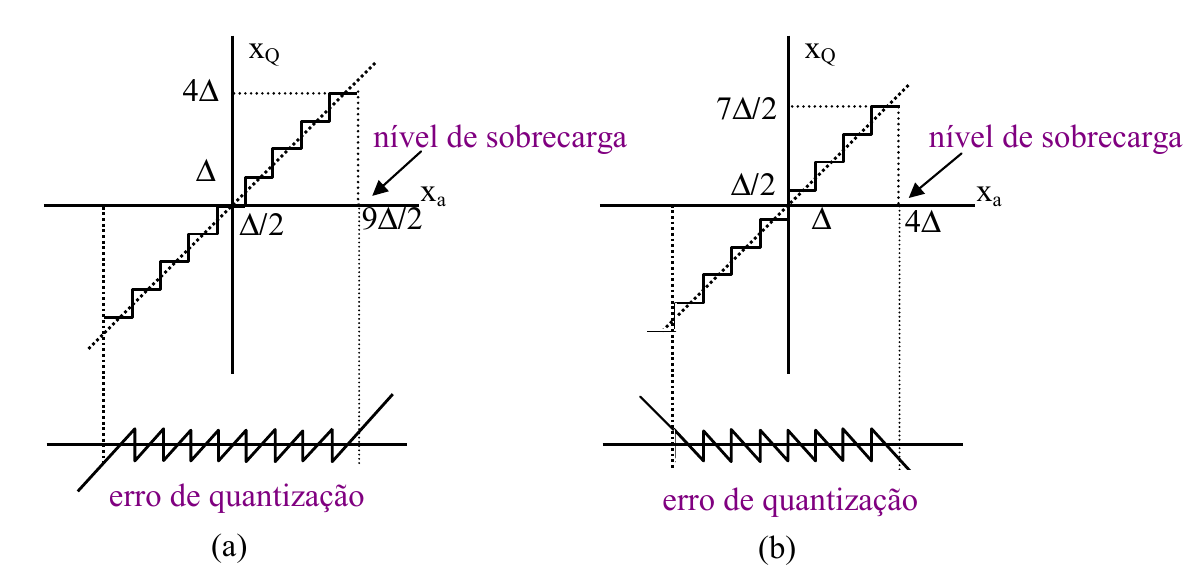
\includegraphics[width = 0.8\linewidth]{img/digital/PCM/QuantizacaoU.png}
    \caption{Características e erro de quantização uniforme: (a) ímpar; (b) par}
    \label{fig:QuantizacaoU}
\end{figure}

\noindent Os dois tipos de característica de quantização ilustradas na \hyperref[fig:QuantizacaoU]{Fig. 7} diferem apenas na forma como cruzam a origem, Formando um número ímpar (\textit{midtread}) ou par (\textit{midrise}) de níveis de quantização (de entrada, $x_a$). Inversamente o passo $\Delta$ dos intervalos de saída, $x_Q$ é par (a) e ímpar (b).
\\
\noindent O número de níveis de quantização em utilização é definido por:
$$
    \boxed{M = \frac{\left|\text{Range}\right|}{\Delta}}
$$
Onde o Range denota o intervalo de amplitudes que o sinal analógico pode tomar. 
\\\\
Subsequentemente, cada um dos $M$ níveis de quantização é codificado por uma palavra de comprimento $L$ onde:
$$
    \boxed{M = n^\text{L}}
$$
Onde $n$ está dependente do sistema PCM em uso (binário: $n = 2$, trenário $n = 3$, quaternário: $n = 4$, ...).

\noindent A geração destas palavras de comprimento $L$ $[$símbolos/sample$]$ não poderá exceder a duração do período de amostragem. É então definido a taxa de geração de dados:
$$
    \boxed{r_s \ge f_s \text{L} \quad [\text{Baud}]}
$$

\noindent onde $f_s$ é a frequência de amostragem e Baud denota a taxa de transmissão de símbolos por segundo.
%adoro-te cutie :3 adoro-te 
%//==============================--@--==============================//%
\paragraph[3.3.1.2 Relação Sinal–Ruído de Quantização]{$\pmb{\star}$ Relação Sinal–Ruído de Quantização}
\mbox{}\\
O erro de quantização definido pela variável aleatória:
$$
    \text{e}(\text{kT}_a) = x_Q(\text{kT}_a) - x_a(\text{kT}_a)
$$
Denomina a diferença entre as amplitudes de entrada e os passos da saída. Tal erro tomará valores que em módulo podem ser muito elevados. De uma forma geral, a discretização das amplitudes de entrada deve ser grande o suficiente de forma a que o o módulo do erro seja sempre inferior a metade do passo:

$$
    \boxed{|\text{e}(\text{kT}_a)| \le \frac{\Delta}{2}}
$$
Para quantificar o desempenho do processo de digitalização–reconstrução usa-se com o medida a relação sinal – ruído de quantização aqui designada por SQNR:
$$
    \boxed{\text{SQNR} = \frac{\text{P}_x}{\text{P}_e}}
$$
em que $P_x$ é a potência do sinal amostrado $x_a(t)$. Para variáveis aleatórias a potência do sinal, é dada por:
$$
    \boxed{P_x = R_x(0) = \text{E}\{x_a(t)^2\} = \int_{-\infty }^{\infty}x^2f(x)\, dx}
$$
onde $f(x)$ é a função de densidade de probabilidade de amplitude.

\vspace{0.5em}
\noindent $P_e$ é a potência do erro, que pode ser aproximado a:
$$
    \boxed{P_e \approx \frac{\Delta^{2}}{12}} 
$$

\noindent É trivialmente concluido que a SQNR diminui quando o comprimento do intervalo de quantização aumenta, o que se traduz numa reconstrução menos precisa do sinal original.

%//==============================--@--==============================//%
\paragraph[3.3.1.3 Quantização Não Uniforme]{$\pmb{\star}$ Quantização Não Uniforme:}
\label{subsubsec:quantizationNU}
A quantização não uniforme visa usar intervalos de quantização mais longos para
amostras que ocorrem em intervalos de menor probabilidade e intervalos de quantização de
menor comprimento no caso contrário. A escolha destes comprimentos deverá portanto ser
feita por forma a otimizar, o desempenho do processo de digitalização–reconstrução.

\vspace{0.5em}
\noindent Esta compressão de intervalos é realizada com base na lei de $\mu$ ou a lei de $A$ (europeia):
\begin{align*}
    |v_\mu| &= \frac{\ln(1 + \mu|m/m_p|)}{\ln(1+\mu)}\text{sgn}(m) &(\mu\textit{-law})\\[6pt]
    |v_A| &= \begin{cases} 
        \dfrac{A |m|}{1 + \ln A}, & |m| \in [0, 1/A] \\[16pt]
        \dfrac{1+\ln(A|m|)}{1+\ln A}, & |m| \in [1/A, 1]
    \end{cases} &(A\textit{-law})
\end{align*}
em que $|m|$ é o \textit{input} normalizado e $|v|$ a saída normalizada.

%//==============================--@--==============================//%
\clearpage
\subsubsection[3.3.2 Gerador de Sinais PCM]{$\rightarrow$ Gerador de Sinais PCM}
\label{subsubsec:arquiteturaPCM}

\begin{figure}[H]
    \centering
    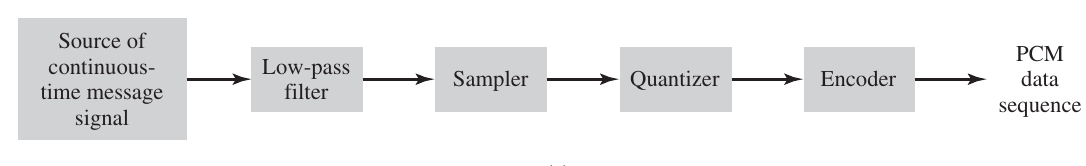
\includegraphics[width = 1\linewidth]{img/digital/PCM/PCM_ARQ.png}
    \caption{Arquitectura do Sistema Gerador de Sinais PCM}
    \label{fig:PCM_ARQ}
\end{figure}

\begin{enumerate}
    \item \textbf{Sampling (amostragem):} O sinal analógico (\textit{continuous-time message signal}) é amostrado com recurso a um pente de pulsos retangulares (\textit{sample and hold}), garantindo um ritmo de amostragem superior ao dobro da componente de frequência mais elevada da mensagem, 2W. (Na prática é utilizado um filtro \textit{antialiasing} ``in order to exclude frequencies greater than W before sampling''\cite{Haykin2007}).
    
    \item \textbf{Quantization (Quantização):} O sinal amostrado é quantizado, tornando-se discreto no tempo e na amplitude (\textit{vide} \hyperref[subsubsec:quantization]{secção sobre a quantização}).
    
    \item \textbf{Encoding:} Posteriormente, o sinal discretizado sofre um ``encoding process to translate the discrete set of sample values to a more appropriate form of signal. Any plan for representing this discrete set of values as a particular arrangement of discrete events is called a code.''\cite{Haykin2007}
\end{enumerate}

\paragraph[3.3.2.1 Line Codes]{$\pmb{\star}$ Line Codes (Códigos de sinalização binária)}
\begin{theo}[\underline{Line Codes} \cite{Haykin2007}]{teo/def:Line Codes}\label{teo/def:LineCodes}
 ``In reality, PCM (...) represent different strategies for source encoding, whereby
an analog signal is converted into digital form. However, all three of them share a common
feature: once a binary sequence of 1s and 0s is produced, a line code is needed for electrical representation of that binary sequence.''
\end{theo}

\noindent De uma forma geral, um código de linha pode ser representado por:
$$
    s(t) = \sum_{n=-\infty}^{\infty} a_n g(t - nT_b)
$$

\noindent Onde $g(t)$ denota a forma do impulso $n$, $a_n$ a sua magnitude e $T_b$ a duração do bit. 

\noindent De uma forma geral, podemos definir o espetro de potência de um código de linha como:
$$
    \boxed{S_s(f) = \frac{|G(f)|^2}{T_b}\sum_{k = -\infty}^{\infty}R(k)e^{j2\pi f k T_b}}\qquad
    \boxed{R(k) = \sum_{i = 1}^{I} a_{n}a_{n+k}p_i}
$$

\noindent Onde $R(0)$ corresponde à potência da sinalização e a largura de banda é definida pelo intervalo de frequências que contem a maior parte da energia do sinal:

$$
    \boxed{B_T = f_T - 0}
$$%miminhos :3 cutie

%//==============================--@--==============================//%
\clearpage
\paragraph*{Unipolar NRZ\protect\footnotemark[2]}\mbox{}\\
\label{line:unipolarNRZ}
\begin{figure}[H]
    \centering
    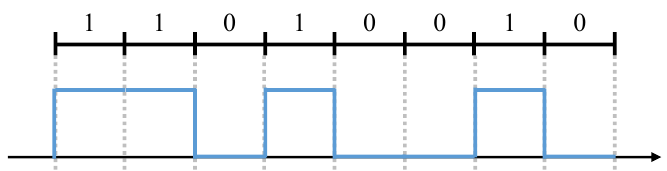
\includegraphics[width = 0.8\linewidth]{img/digital/line-codes/LUnipolarNRZ.png}
    \caption{Unipolar NRZ (11010010).}
    \label{fig:LUnipolarNRZ}
\end{figure}
\noindent Um código unipolar NRZ possui pulsos do tipo:
$$
    g(t) = \text{rect}\left(\frac{t}{T_b}\right)
$$
\noindent Com o respetivo espetro de potência:

$$
    \boxed{S_s(f) = \frac{A^2 T_b}{4}\, \text{sinc}(fT_b)^2\left[1 + \frac{1}{T_b}\delta(f)\right]}
$$

\noindent E potência e largura de banda (supondo que o sinal atinge a grande maioria da sua energia após o primeiro zero do espetro de potência):
%adoro-te
\begin{figure}[H]
    \centering
    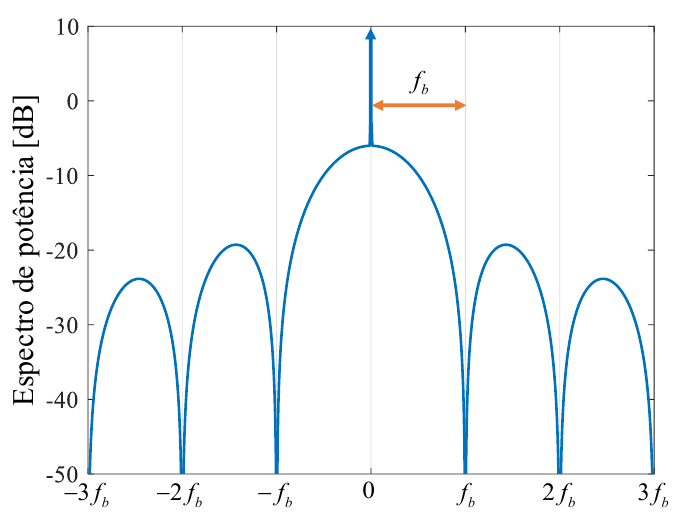
\includegraphics[width = 0.7\linewidth]{img/digital/line-codes/PUnipolarNRZ.png}
    \caption{Espetro de Potência unipolar NRZ.}
    \label{fig:PUnipolarNRZ}
\end{figure}

$$
    \boxed{P = R(0) = A^2}\qquad
    \boxed{B_T = f_{\text{1º zero}} - 0 = \frac{1}{T_b}}
$$

\footnotetext[2]{A vizualização dos códigos de sinalização binária subsequente no domínio do tempo será realizada mediante o código 11010010.}

%//==============================--@--==============================//%
\clearpage
\paragraph*{Unipolar RZ}\mbox{}\\
\label{line:unipolarRZ}
\begin{figure}[H]
    \centering
    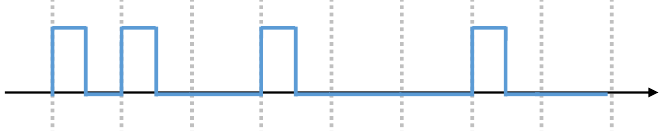
\includegraphics[width = 0.8\linewidth]{img/digital/line-codes/LUnipolarRZ.png}
    \caption{Unipolar NRZ (11010010).}
    \label{fig:LUnipolarRZ}
\end{figure}
\noindent Um código unipolar RZ (com um \textit{duty-cycle} de $50\%$) possui pulsos do tipo:
$$
    g(t) = \text{rect}\left(\frac{2t}{T_b}\right)
$$
\noindent Com o respetivo espetro de potência:

$$
    \boxed{S_s(f) = \frac{A^2 T_b}{16}\, \text{sinc}(fT_b/2)^2\left[1 + \frac{1}{T_b}\sum_{k = -\infty}^{k = \infty}\delta(f-kT_b/2)\right]}
$$

\noindent E potência e largura de banda (supondo que o sinal atinge a grande maioria da sua energia após o primeiro zero do espetro de potência):

\begin{figure}[H]
    \centering
    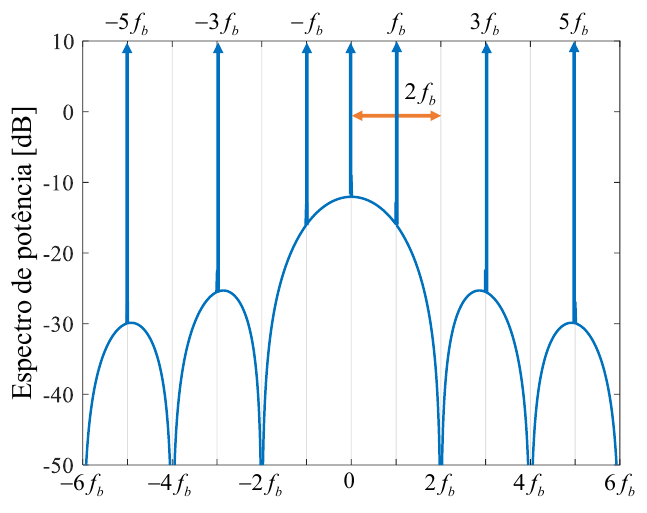
\includegraphics[width = 0.7\linewidth]{img/digital/line-codes/PUnipolarRZ.png}
    \caption{Espetro de Potência unipolar RZ.}
    \label{fig:PUnipolarRZ}
\end{figure}

$$
    \boxed{P = R(0) = \frac{A^2}{4}}\qquad
    \boxed{B_T = f_{\text{1º zero}} - 0 = \frac{2}{T_b}}
$$

\noindent A potência média deste código será de metade do código Unipolar NRZ, uma vez que, é emitida a mesma energia, nos símbolos com amplitude maior que zero, mas em metade do tempo.
%//==============================--@--==============================//%
\clearpage
\paragraph*{Polar NRZ}\mbox{}\\
\label{line:polarNRZ}
\begin{figure}[H]
    \centering
    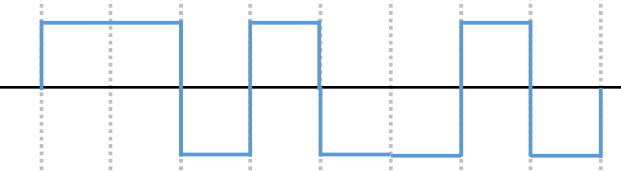
\includegraphics[width = 0.8\linewidth]{img/digital/line-codes/LPolarNRZ.png}
    \caption{Polar NRZ (11010010).}
    \label{fig:polarNRZ}
\end{figure}
\noindent Um código Polar NRZ possui pulsos do tipo:
$$
    g(t) = \text{rect}\left(\frac{t}{T_b}\right)
$$
\noindent Com o respetivo espetro de potência:

$$
    \boxed{S_s(f) = A^2 T_b\, \text{sinc}(fT_b)^2}
$$

\noindent E potência e largura de banda (supondo que o sinal atinge a grande maioria da sua energia após o primeiro zero do espetro de potência):

\begin{figure}[H]
    \centering
    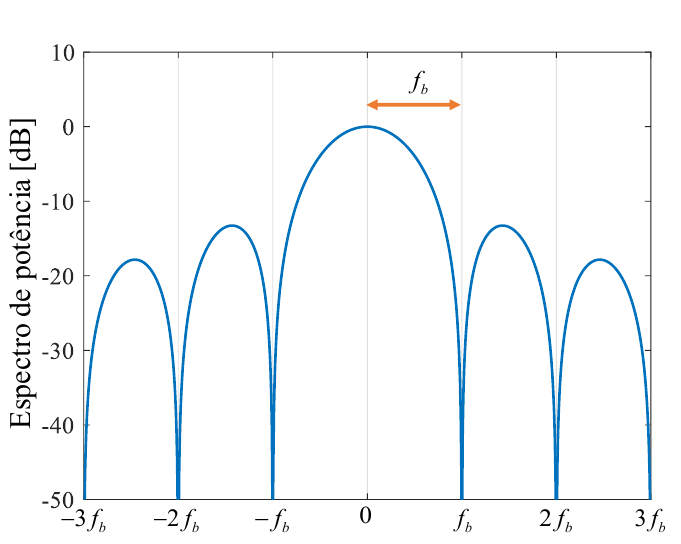
\includegraphics[width = 0.7\linewidth]{img/digital/line-codes/PPolarNRZ.png}
    \caption{Espetro de Potência polar NRZ.}
    \label{fig:PpolarNRZ}
\end{figure}

$$
    \boxed{P = R(0) = A^2}\qquad
    \boxed{B_T = f_{\text{1º zero}} - 0 = \frac{1}{T_b}}
$$
%//==============================--@--==============================//%
\clearpage
\paragraph*{Polar RZ}\mbox{}\\
\label{line:polarRZ}
\begin{figure}[H]
    \centering
    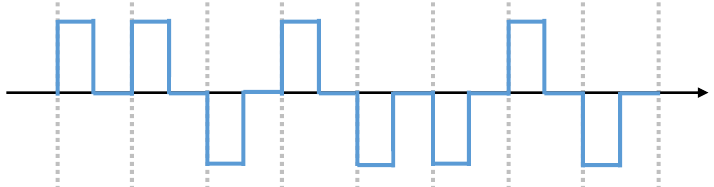
\includegraphics[width = 0.8\linewidth]{img/digital/line-codes/LPolarRZ.png}
    \caption{Polar RZ (11010010).}
    \label{fig:LPolarRZ}
\end{figure}
\noindent Um código Polar RZ (com um \textit{duty-cycle} de $50\%$) possui pulsos do tipo:
$$
    g(t) = \text{rect}\left(\frac{t}{2T_b}\right)
$$
\noindent Com o respetivo espetro de potência:

$$
    \boxed{S_s(f) = \frac{A^2 T_b}{4}\, \text{sinc}(fT_b)^2}
$$

\noindent E potência e largura de banda (supondo que o sinal atinge a grande maioria da sua energia após o primeiro zero do espetro de potência):

\begin{figure}[H]
    \centering
    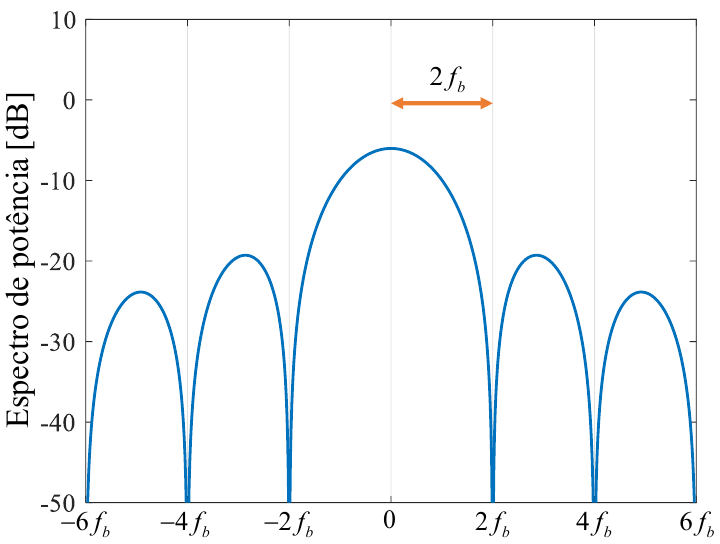
\includegraphics[width = 0.7\linewidth]{img/digital/line-codes/PPolarRZ.png}
    \caption{Espetro de Potência: Polar RZ.}
    \label{fig:PPolarRZ}
\end{figure}

$$
    \boxed{P = R(0) = \frac{A^2}{2}}\qquad
    \boxed{B_T = f_{\text{1º zero}} - 0 = \frac{2}{T_b}}
$$

%//==============================--@--==============================//%
\clearpage
\paragraph*{Bipolar NRZ}\mbox{}\\
\label{line:bipolarNRZ}
\begin{figure}[H]
    \centering
    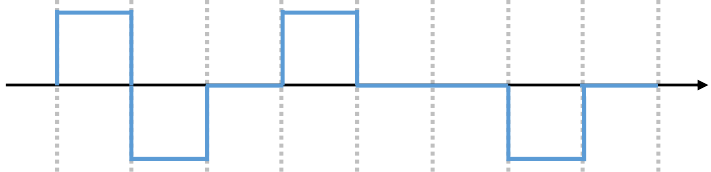
\includegraphics[width = 0.8\linewidth]{img/digital/line-codes/LBipolarNRZ.png}
    \caption{Bipolar NRZ (11010010).}
    \label{fig:bipolarNRZ}
\end{figure}
\noindent Um código Bipolar NRZ possui pulsos do tipo:
$$
    g(t) = \text{rect}\left(\frac{t}{T_b}\right)
$$
\noindent Com o respetivo espetro de potência:

$$
    \boxed{ S_s(f) = \frac{A^2 T_b}{2} \left[\text{sinc}(f T_b)\right]^2 \cdot \left[\sin(\pi f T_b)\right]^2 }
$$

\noindent E potência e largura de banda (supondo que o sinal atinge a grande maioria da sua energia após o primeiro zero do espetro de potência):

\begin{figure}[H]
    \centering
    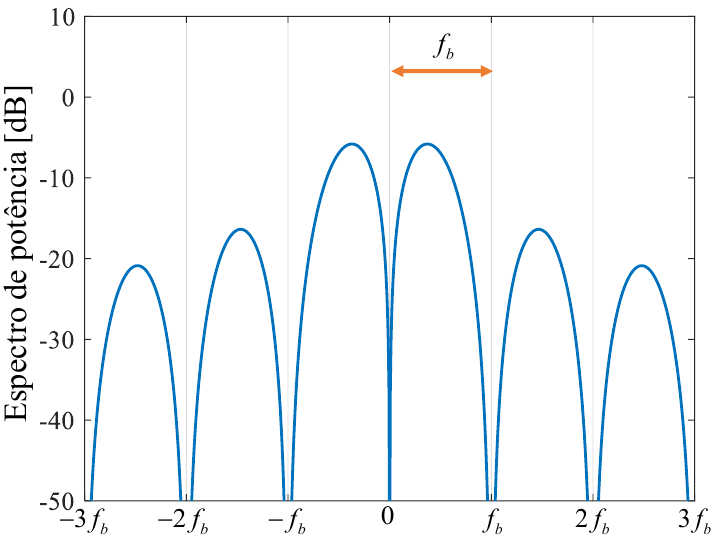
\includegraphics[width = 0.7\linewidth]{img/digital/line-codes/PBipolarNRZ.png}
    \caption{Espetro de Potência: Bipolar NRZ.}
    \label{fig:PBipolarNRZ}
\end{figure}

$$
    \boxed{P = R(0) = \frac{A^2}{2}}\qquad
    \boxed{B_T = f_{\text{1º zero}} - 0 = \frac{1}{T_b}}
$$

%//==============================--@--==============================//%
\clearpage
\paragraph*{Bipolar RZ}\mbox{}\\
\label{line:bipolarRZ}
\begin{figure}[H]
    \centering
    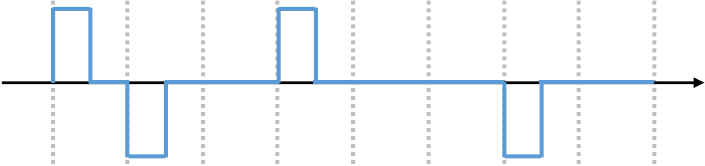
\includegraphics[width = 0.8\linewidth]{img/digital/line-codes/LBipolarRZ.png}
    \caption{Bipolar RZ (11010010).}
    \label{fig:bipolarRZ}
\end{figure}
\noindent Um código Bipolar RZ (com um \textit{duty-cycle} de $50\%$) possui pulsos do tipo:
$$
    g(t) = \text{rect}\left(\frac{t}{2T_b}\right)
$$
\noindent Com o respetivo espetro de potência:

$$
    \boxed{ S_s(f) = \frac{A^2 T_b}{8}\, \left[\text{sinc}(f\frac{T_b}{2})\right]^2 \cdot \left[\sin(\pi f \frac{T_b}{2})\right]^2 }
$$

\noindent E potência e largura de banda (supondo que o sinal atinge a grande maioria da sua energia após o primeiro zero do espetro de potência):

\begin{figure}[H]
    \centering
    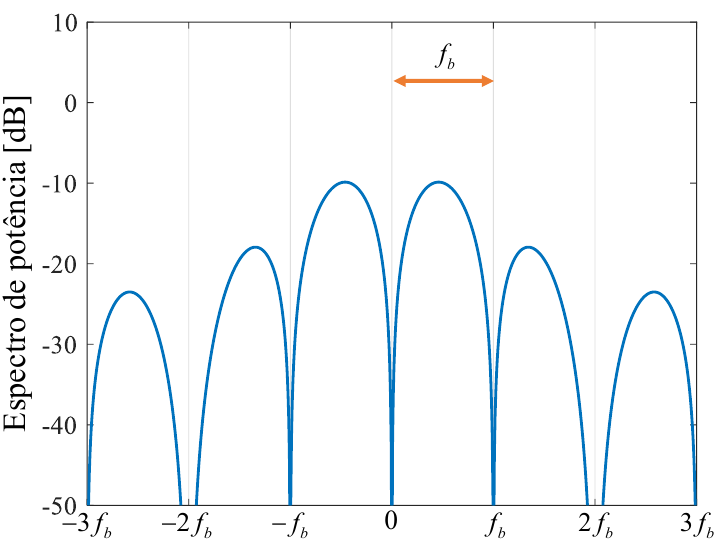
\includegraphics[width = 0.7\linewidth]{img/digital/line-codes/PBipolarRZ.png}
    \caption{Espetro de Potência polar NRZ.}
    \label{fig:PBipolarRZ}
\end{figure}

$$
    \boxed{P = R(0) = \frac{A^2}{4}}\qquad
    \boxed{B_T = f_{\text{1º zero}} - 0 = \frac{1}{T_b}}
$$

%//==============================--@--==============================//%
\clearpage
\paragraph*{Manchester}\mbox{}\\
\label{line:manchester}
\begin{figure}[H]
    \centering
    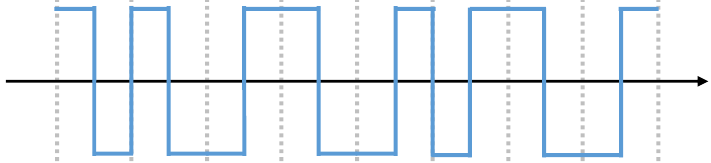
\includegraphics[width = 0.8\linewidth]{img/digital/line-codes/LManchester.png}
    \caption{Manchester (11010010).}
    \label{fig:manchester}
\end{figure}
\noindent Um código Manchester possui pulsos do tipo:
$$
    g(t) = \text{rect}\left(\frac{t+T_b/4}{2T_b}\right) - \text{rect}\left(\frac{t - T_b/4}{2T_b}\right) 
$$
\noindent Com o respetivo espetro de potência:

$$
    \boxed{S_s(f) = A^2 T_b\, \left[\text{sinc}(f\frac{T_b}{2})\right]^2 \cdot \left[\sin(\pi f \frac{T_b}{2})\right]^2 }
$$

\noindent E potência e largura de banda (supondo que o sinal atinge a grande maioria da sua energia após o primeiro zero do espetro de potência):

\begin{figure}[H]
    \centering
    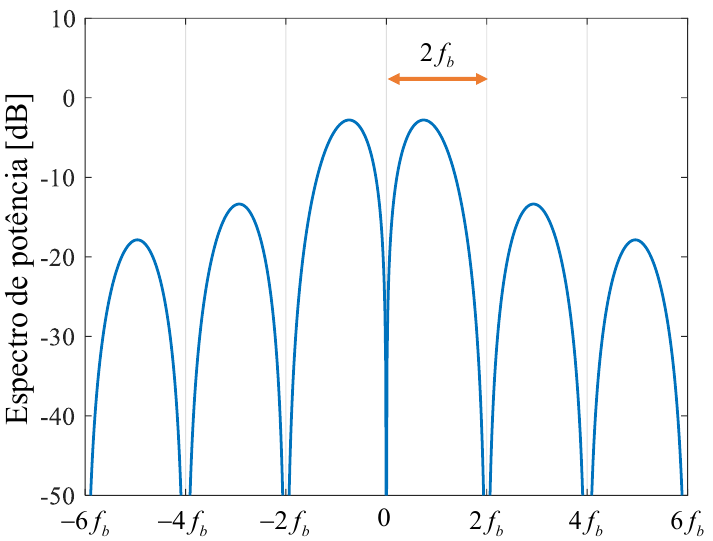
\includegraphics[width = 0.7\linewidth]{img/digital/line-codes/PManchester.png}
    \caption{Espetro de Potência: Manchester.}
    \label{fig:PManchester}
\end{figure}

$$
    \boxed{P = R(0) = A^2}\qquad
    \boxed{B_T = f_{\text{1º zero}} - 0 = \frac{2}{T_b}}
$$
%//==============================--@--==============================//%